\chapterimage{./Pictures/cover-shell} % Chapter heading image
\chapter{TP1 : Manipulations de l’environnement et des fichiers sous UNIX}

\section{Exercice 1 : Découverte de quelques commandes d'archivage}
\textit{L'objectif de cet exercice est de découvrir et manipuler les commandes de téléchargement, d'archivage, de compression et de décompression de fichier}

\paragraph{1. Récupération et décompression d'une archive}
La commande \texttt{wget https://cloud.infotro.fr/ITC313/archive.tar} permet de télécharger l'archive présent à cette adresse.
\begin{itemize}
\item L'option \texttt{-x} permet de restaurer les fichiers contenus dans une archive.
\item L'option \texttt{-c} permet de créer une nouvelle archive.
\item L'option \texttt{-f} permet d'utilise le fichier archive F ou le périphérique F (par défaut /dev/rmt0).
\end{itemize}
9 fichiers était présent dans cette archive

\paragraph{2. Manipulation de fichiers}
\texttt{file .\/*}
Afin de renommer le fichier j'utilise cette commande \texttt{mv image4.jpg image4.jpg2}.
Le fichier \texttt{script.txt} fait 170Ko.
La commande \texttt{gzip} sur \texttt{script.txt} a compressé le fichier.
Le fichier fait maintenant  65Ko.
La compréssion est donc d'environ 38.235\%.
Après décompression avec la commande \texttt{gunzip} le fichier fait maintenant 170Ko, qui est la taille initial du fichier.

\paragraph{3. Création d'une nouvelle archive}
La nouvelle archive fait 850Ko soit 1Ko de moins que l'ancienne archive. Surement à cause du nom de fichier jp2 changé.
La somme des tailles des fichiers dans l'archive est égale à 845479 soit 845Ko, on observe une différence de 5Ko.
La compression de l'archive (créé précédemment) fait 617Ko soit une différence de 228Ko.
L'option \texttt{-z} utilise gzip pour comprésser l'archive.
Elle revient totalement à créé une archive puis la compresser puisque d'après les test la taille n'est pas différente.
La Commande \texttt{tar -c -z *.jpg *.txt *.jp2} devrait normalement afficher dans le terminal le résultat.
La Commande \texttt{tar -c -z *.jpg *.txt *.jp2 > nouvelleArchive3.tar.gz} redirige bien le résultat dans un fichier.
La redirection du flux dans un fichier recréer une archive compréssé similaire à la deuxième créé.
En conclusion l'archive 2 et 3 donne le même résultat et sont plus petit que l'archive 1 puisqu'elles sont compréssés.

\section{Exercice 2 : Utilisation des masques de création de fichiers}
\begin{figure}[!h]
\centering
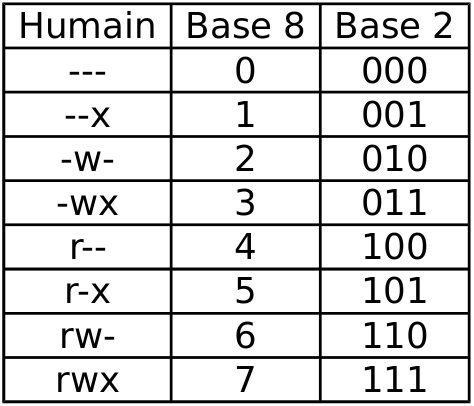
\includegraphics[width=250pt]{./shell/Pictures/permissions}
\caption{Permissions Unix}
\label{Permissions Unix}
\end{figure}

\paragraph{1.}
\begin{minted}{shell}
touch Raphael.txt
umask 0666
touch Donatello.txt
umask 0331
touch Michelangelo.txt
umask 0661
touch Leonardo.txt
umask 0000
\end{minted}

\paragraph{2. et 3.}
Il n'est pas possible de créer de donner plus de droit que la limitation par défaut du systeme.
( application umask par défaut 666 sur fichier et 777 sur repertoire)

\section{Exercice 3 : Manipulation du Systeme de fichier et des droits de navigation}

\paragraph{1.}
L'archive contient 5 images.

\paragraph{3.}
\mintinline{shell}{/home/ESIREM-AD/al669724/Documents/Shell/TPs/TP1/Ex3/images/Chinpokomon/P-Z/Vamporc.png}

\paragraph{4.}
\mintinline{shell}{../P-Z/Vamporc.png}

\paragraph{6.}
L'option \texttt{-z} permet de compresser l'archive.
\mintinline{s}{tar -xczf ITC313_TP_Shelllebot.axel.tar.gz}
permettra de décompresser et extraire l'archive.

\paragraph{7.}
Toutes les permissions sont conservés.

\section{Exercice 4 : Manipulation d'expression régulière}

\paragraph{2.}
Les lignes contenant la suite de lettres "ette".

\paragraph{3.}
Les lignes contenant la lettre "T".

\paragraph{4.}
Les lignes commencant par la lettre "T".

\paragraph{5.}
\texttt{\^} signifie "début".

\paragraph{6.}
Les lignes finissant par "te".

\paragraph{7.}
Les lignes contenant la suite de caractère "c", un caractère, "r".

\paragraph{8.}
Les lignes contenant "oui" ou "non".

\paragraph{9.}
\begin{itemize}
\item '\$' -> en fin
\item '|' -> ou
\item '.' -> un caractère
\end{itemize}

\paragraph{10.}
Permet d'afficher uniauement la partie correspondant à la recherche.

\paragraph{11.}
Une suite de 4 lettre Majuscule.

\paragraph{12.}
Une suite d'au moins une Majuscule et un minuscule

\paragraph{13.}
Les mots commencant par une majuscule aisni que les lettre majuscules.

\paragraph{15.}
Permet de récupérer les addresse e-mail.

\paragraph{16.}
Permet de récupérer les numéro de téléphone.

\paragraph{17.}
((bien))((joue))((tu))((as))((trouve))((la))((reponse))((a))((la))((derniere))((question))
